
\section{Resolución SLD}
Si bien los métodos que propusimos hasta ahora son completos, hallar refutaciones es un proceso muy car en el caso general, el espacio de búsqueda que producen puede ser enorme y tienen un alto grado de no-determinismo. Debemos agregar ciertas restricciones que nos permitan reducir este espacio sin que esto afecte a la completitud del método.

\subsection{Resolución lineal}
Una secuencia de pasos de resolución a partir de $S$ es \textbf{lineal} si es de la forma:

\begin{center}
	\begin{forest} resolucion,
[$C_p~{=}~\Box$ 
	[$C_{p-1}$,edge label={node[midway,right] {$\blue{\sigma_p}$}}
    	[$\dots$,edge label={node[midway,right] {$\blue{\sigma_{p-1}}$}}
        	[$C_3$,
            	[$C_2$,edge label={node[midway,right] {$\blue{\sigma_3}$}}
                	[$C_1$, edge label={node[midway,right] {$\blue{\sigma_2}$}}
           	        	[$C_0$, edge label={node[midway,right] {$\blue{\sigma_1}$}}]
                      	[$B_1$]
                	]
                	[$B_2$]        	
            	]
                [$B_3$]
        	]
    	]
    	[$B_{p-1}$]	
	]
    [$B_p$]
]
	\end{forest}
\end{center}

donde $C_0$ y cada $B_i$ es un elemento de $S$ o algún $C_j$ con $j < i$.

Este tipo de resolución reduce el espacio de búsqueda considerablemente, sin embargo sigue siendo altamanente no-deterministico ya que no se se especificó ningún criterio de búsqueda ni selección de las cláusulas que debemos usar de este espacio.

\subsection{Cláusulas de Horn}
Podemos lograr una mayor eficiencia en el proceso de producir refutaciones si solo consideramos una \textbf{subclase} de fórmulas lo suficientemente expresivas. Es decir, que si bien existirán fórmulas que no podremos resolver con este método, las fórmulas que resolveremos tendrán el suficiente poder como para ser un método computacionalmente completo.

El subconjunto de clásulas que vamos a usar son las cláusulas de Horne:

Una cláusula $\forall x_1\dots\forall x_m.C$ tal que la disyunción de literales $C$ tiene \textbf{a lo sumo} un literal positivo. Y diremos que una cláusula de esta forma es una \textbf{cláusula de definición} cuando $C$ tiene \textbf{exactamente} un literal positivo.

El método de resolución SLD, tendrá como entrada un conjunto de cláusulas de Horn $S = P\cup \{G\} $ donde $P$ es nuestro programa (conjunto de axiomas y reglas de entrada o base de conocimiento) y $G$ es nuestro goal.

Una secuencia de pasos de \textbf{resolución SLD} para $S$ es una secuencia $<N_0,N_1,\dots, N_p>$ de \textbf{cláusulas negativas} que satisfacen las siguientes dos condiciones:
\begin{enumerate}
\item $N_0$ es el goal $G$.
\item para todo $N_i$ en la secuencia, $0 < i < p$, si $N_i$ es 
$$\{\lnot A_1,\dots, \lnot A_{k-1}, \lnot A_{k}, \lnot A_{k+1},\dots, \lnot A_n\}$$
entonces hay alguna \textbf{cláusula de definición} $C_i$ de la forma $\{A,\lnot B_1,\dots, \lnot B_m\}$ en $P$ tal que $A_k$ y $A$ son unificable con el MGU $\sigma$ y si :
\begin{itemize}
\item $m = 0$, entonces $N_{i+1}E$ es
$$\{ \sigma(\{\lnot A_1,\dots, \lnot A_{k-1}, \lnot A_{k+1},\dots, \lnot A_n\}) \}$$
\item $m > 0$, entonces $N_{i+1}E$ es
$$\{ \sigma(\{\lnot A_1,\dots, \lnot A_{k-1}, \lnot B_1,\dots, \lnot B_m, \lnot A_{k+1},\dots, \lnot A_n\}) \}$$
\end{itemize}
\end{enumerate}

Esto significa que cada paso de la secuencia es la resolución del pase anterior con una cláusula de Horne definida en nuestro programa que tiene un literal positivo $A$ que unifica con algún literal $A_k$ negado en dicho paso. Llamaremos \textbf{átomo seleccionado} al literal $A_k$. Y \textbf{sustitución respuesta} a la composición de las sustituciones.

Este es el método que usa Prolog para extraer la salida del programa. Por ejemplo, si consideramom el siguiente programa:

\begin{itemize}
\item $C_1 = \{add(U,O,U)\}$
\item $C_1 = \{add(X,succ(Y),succ(Z), \lnot add(X,Y,Z)\}$
\end{itemize}

Y definimos nuestro goal $G = \{\lnot add(succ(0),V,succ(succ(0))))\}$, entonces una resolución posible es la siguiente:

\begin{center}
	\begin{forest} resolucion,
[$\Box$ 
	[$\{\lnot add(succ(0){,}~V{,}~succ(succ(0))\}$,edge label={node[midway,right] {$\sigma_2$}}
    	[$\{\lnot add(succ(0){,}V{,}succ(succ(0))))\}$,edge label={node[midway,right] {$\sigma_1$}}
    	]
    	[$C_2$]	
	]
    [$C_1$]
]
	\end{forest}
\end{center}

$\sigma_1 = \{ X\leftarrow succ(0),~Z\leftarrow succ(0),~ V\leftarrow succ(Y)\}$

$\sigma_2 = \{ U\leftarrow succ(0),~Y\leftarrow 0\}$

Y la sustitución resultado es: $$\{ X\leftarrow succ(0),~Z\leftarrow succ(0),~ V\leftarrow succ(0),U\leftarrow succ(0),~Y\leftarrow 0\}$$

\subsubsection{Corrección y completitud}

\paragraph{Corrección} Si un conjunto de cláusulas de Horn tiene una refutación SLD, entonces es insatisfactible.

\paragraph{Completitud} Dado un conjunto de cláusulas de Horn $P\cup \{G\}$, si $P\cup \{G\}$ es insatisfactible, existe una refutación SLD cuya primera cláusula es $G$.

\subsection{Resolución SLD en Prolog}
El método SLD todavía deja sin determinar como realizar la búsqueda y la selección de las cláusulas de nuestro programa para aplicar en la resolución. Para solucionar esto, se usan \textbf{estrategias} que determinan la forma de los árboles de búsqueda o \textbf{árbol SLD} de nuestra resolución.


Esto quiere decir que cuando diseñamos un programa debemos tener en cuenta la estrategia que estamos usando para determinar el orden de las cláusulas que estamos definiendo. Hay que tratar de que el método consiga, primero, las soluciones de las ramas ``mas interesante'' y luego explore el resto del árbol.

Podría llegar a pasarnos que, debido a una mala elección de este orden (para la estrategia elegida), el método no encuentre una refutación para una expresión que es insatisfactible. 

Prolog, en particular, selecciona las cláusulas del programa de arriba hacia abajo, es decir, en el orden en que fueron introducidas y el átomo seleccionado en cada paso es el átomo de más a la izquierda de la fórmula. Además, como puede haber varias resoluciones SLD, Prolog realiza backtracking sobre las reglas usadas para generar todas las soluciones posibles.
Si consideramos el siguiente programa:

\begin{enumerate}
\item $\{ p(X,Z),~\lnot q(X,Y), \lnot p(Y,Z) \}$
\item $\{ p(X,X)\}$
\item $\{q(a,b)\}$
\end{enumerate}

Y nuestro goal es $\{\lnot p(X,b)\}$, entonces, Prolog, realizaría el siguiente árobl SLD:

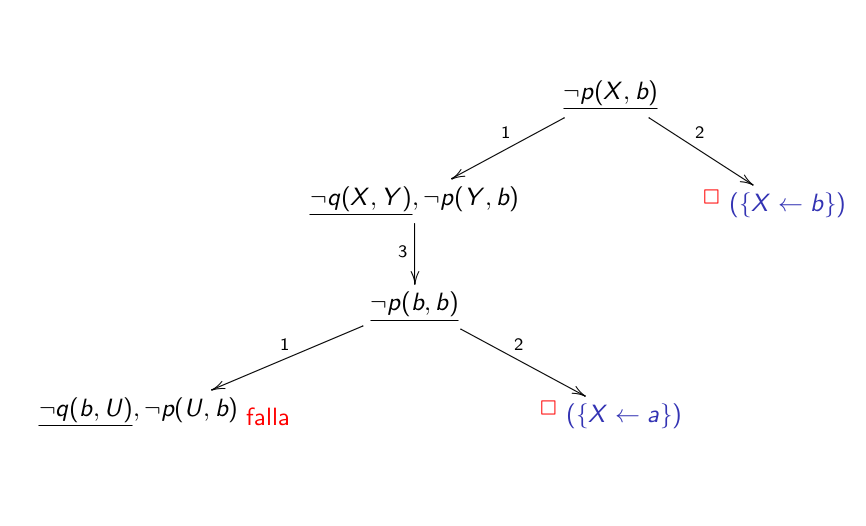
\includegraphics[scale=0.4]{imagenes/arbol_sld_prolog.png}

Otra posible estrategia de selección sería, por ejemplo, elegir resolver la cláusula más a la derecha, en cuyo caso el ejemplo que dimos dejaría de funcionar ya que la primer rama del árbol sería infinita y no encontrariamos nunca una refutación.

Y si decidiesemos seleccionar las cláusulas de abajo hacia arriba, entonces obtendriamos el árbol mostrado reflejado.

Hay que tener en cuenta que elegimos el ejemplo para que funcionase bien con la estrategia que sigue Prolog, sin embargo, hay ejemplos en lo que esta estrategia cae en el mismo caso que en la primer estrategia alternativa mencionada.

\subsubsection{Implementación y otras cosas sobre Prolog}
La estrategia usada por Prolog recorre el árbol SLD en \textbf{profundidad} (depth-first search). Las ventajas de esto es que puede ser implmentado de manera muy eficiente usando una \textbf{pila} para representar los átomos del goal.
La idea es hacer un \textbf{push} del resolvente del átomo del tope de la pila con la cláusula de definición y hacer un \textbf{pop} cuando el átomo del top de la pila no unifica con ninguna cláusula de definición más.

\subsubsection*{Cut}
Es una notación que nos permite \textbf{podar} el árbol SLD. Es de carácter extra-lógico y nos permite \textbf{hacer más eficientes} algunas consultas. El uso correcto de esta notación no debería modificar el universo de posibles soluciones a una consulta.

Cuando se selecciona un cut, tiene éxito \textbf{inmediatamente}. Si, debido a backtracking, se vuelve al mismo cut entonces se hace fallar el goal que le dio origen.

\subsection*{Negación por falla}
Se dice que un árbol SLD \textbf{falla finitamente} si es finito y no tiene ramas de éxito.

Dado un programa P el \textbf{conjunto de falla finita} de $P$ es $$\{ B ~|~B~ \text{ es un átomo cerrado y existe un árbol SLD que falla finitamente con } B \text{ como raíz}\} $$ 

Esto significa que podemos inferir la insatisfactibilidad de una cláusula cerrada si la cantidad de chequeos que tenemos que hacer para probarlo es finita y si, además, tenemos un conjunto finito de símbolos sobre los que chequear.

En Prolog, tenemos el predicado \textbf{not} que nos permite realizar este tipo de resolución, sin embargo debemos asegurarnos de que los predicados que le pasemos sean cerrados, ya que al no ser un predicado lógico, no se instancias variables en ningún momento.